\chapter{Bausteinsicht}
\label{sec:bausteine}
Die Bausteinsicht ist der Grundrissplan einer jeden Software. Für die Anwendung eCourse ist die Bausteinsicht in Abbildung \ref{fib:Bausteinsicht} dargestellt.
Diese Darstellung ist eine statische Zerlegung des Systems in Bausteine. Diese Ansicht ermöglicht es vor allem die Kommunikation zwischen den Entwicklern untereinander bzw. mit dem Stakeholder zu erleichtern, da sie das System abstrahiert und dadurch von der Besprechung von Implementierungsdetails entbindet.

\begin{figure}[H]
\centering
\includegraphics[height=1.0\textwidth]{bausteinsicht.png}
\caption{Bausteinsicht für die Anwendung eCourse}
\label{fib:Bausteinsicht}
\end{figure}

\section{Gesamtsystem}
Durch eCourse soll es \gls{Studierende}n und \gls{Dozierende}n möglich sein Dateien untereinander auszutauschen. Ebenso soll den Verwaltungsangestellten Einblick in die ausgetauschten Dateien ermöglicht werden, um bei Bedarf verwaltende Tätigkeiten ausführen zu können. Diese drei Benutzergruppen greifen direkt auf die Anwendung eCourse zu. Es gibt keine weiteren Schnittstellen zu anderen Anwendungen, wie in Kapitel \ref{sec:kontext} bereits erläutert wurde. 

\section{Überblick}
Blickt man genauer in die Anwendung eCourse hinein, ergibt sich eine Aufteilung in \gls{Backend} und \gls{Frontend}.

\subsection{Frontend}
Das \gls{Frontend} beschreibt dabei den Teil der Anwendung, der näher am Nutzer liegt. Folglich ist es die Schnittstelle zwischen Nutzer und der dahinter liegenden Logik der Anwendung. Alle drei Nutzergruppen haben Zugriff auf das \gls{Frontend}, wobei durch das \gls{Frontend} abhängig von der Nutzergruppe unterschiedliche Informationen und Funktionen präsentiert werden. Eine genaue Darstellung der Rechte die die jeweilige Nutzergruppe hat ist in \ref{fib:erlaubnis} zu finden.

\subsection{Backend}
Das \gls{Backend} ist dann im Gegensatz zum \gls{Frontend} die Logik hinter der Anwendung. Hier werden die Ergebnisse jeder Nutzerinteraktion berechnet. Genauere Details zum \gls{Backend} finden sich in Kapitel \ref{sec:Datenbank} und \ref{sec:Server}.

\section{Detail}

\subsection{WebInterface}
Das \gls{Frontend} besteht im Wesentlichen aus einem \gls{Webinterface}. Über eine Webseite, die als \gls{Webinterface} dient, können die Benutzer verschiedene Aktivitäten ausführen. Abhängig davon, welcher Gruppe der Benutzer angehört sind unterschiedliche Aktionen möglich. 
Diese Aktivitäten sind in Abbildung \ref{fib:erlaubnis} dargestellt.

\begin{figure}[H]
\centering
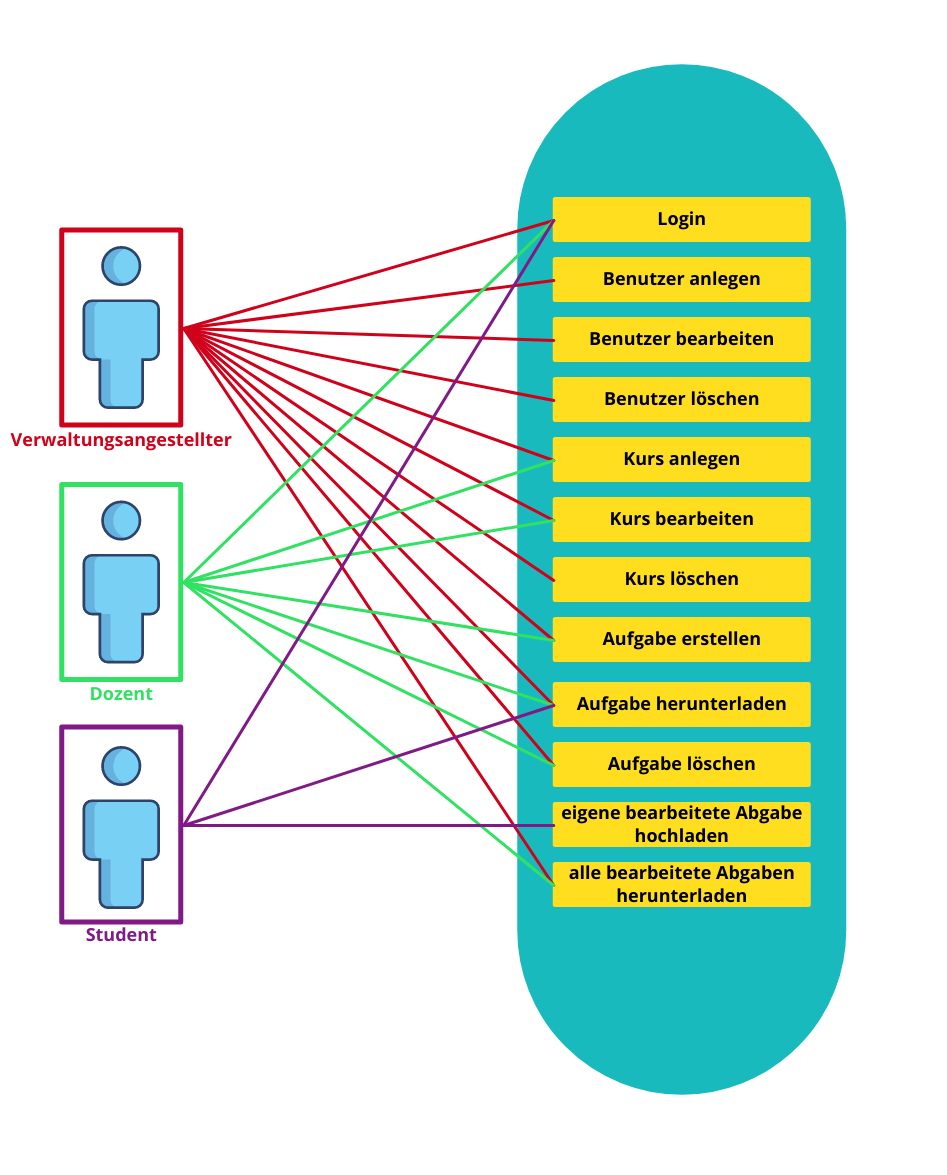
\includegraphics[height=1.0\textwidth]{erlaubnisdiagramm.png}
\caption{Erlaubnisdiagramm für die Anwendung eCourse}
\label{fib:erlaubnis}
\end{figure}

\subsection{Datenbank}
\label{sec:Datenbank}

An das Backend ist eine SQL-Datenbank zur Datenhaltung angeschlossen. Dort werden die Stammdaten der Nutzenden, sowie die Daten der Kurse gespeichert. Zu Entwicklungszwecken wurde anfangs auf die Datenbanksoftware \glqq SQLite\grqq\; aufgrund ihrer Einfachheit gesetzt. Aufgrund der Verwendung eines DBMS ist das Wechseln auf eine andere SQL-Datenbank in der Konfiguration möglich. Dies ist in dem Dokument \enquote{Planung von Wartung und Betrieb} beschrieben.
Die Datenbank ist ausschließlich zur Datenhaltung bestimmt und enthält keine Geschäftslogik. Diese ist außerhalb der Datenbank implementiert


\subsection{Server}
\label{sec:Server}
Die Geschäftslogik der Anwendung ist als Django Applikation verwirklicht. Die Logik selbst ist dabei in einige gekapselte Module aufgespalten, jene die Wartbarkeit und Erweiterbarkeit der Software erhöhen sollen. In Tabelle \ref{tab:module} ist eine Auflistung der Module mitsamt einer kurzen Beschreibung enthalten.


\begin{table}[H]
\centering
\begin{tabularx}{\textwidth}[H]{|X|X|}
\hline
Modulname & Kurzbeschreibung\\
\hline
eCourse\_backend & Programmeinstiegspunkt\\
\hline
users & Benutzerverwaltung \\
\hline
courses & Kursverwaltung \\
\hline
file\_exchange & Aufgabenstellungs- und Abgabenlogik \\
\hline
\end{tabularx}
\caption{Module des Backends der Anwendung eCourse}
\label{tab:module}
\end{table}

Der Programmeinstiegspunkt übernimmt die Aufgabe des Weiterleitens der Anfragen auf das zuständige Modul.
